%-*- coding: UTF-8 -*-
% MathGraphs.tex
%
\documentclass[UTF8]{ctexart}
\usepackage{geometry}
\geometry{a4paper, centering, scale=0.8}
\usepackage{minted}
\usepackage{float}
\usepackage{amsmath}
\usepackage{tikz}
\usepackage{hyperref}

\title{\heiti 第5章 \quad 数学插图}
\author{\kaishu Du Ang \\ \texttt{du2ang233@gmail.com} }
\date{\today}


\begin{document}
\maketitle

\tableofcontents

\newpage

\section{概述}
除了排版文字,\LaTeX 也支持用代码表示图形。\LaTeX 提供了原始的 \texttt{picture} 环境,能够绘制一些基本的图形如
点、线、矩形、圆等等。不过受制于 \LaTeX 本身,它的绘图功能极为有限,效果也不够美观。

不同的扩展极大地丰富了 \LaTeX 的图形功能,TikZ 就是其中之一。一些特殊的绘图,如交换图、树状图甚至分子式和电路图也能
够通过代码绘制,不过过于复杂。

现在流行的绘图代码有以下几种:
\begin{itemize}
    \item PSTricks \\ 以 PostScript 语言的功能为基础的绘图宏包,具有优秀的绘图能力。它对老式的
    \texttt{latex + dvips} 编译命令支持最好,而现在的几种编译命令下使用起来都不够方便。
    \item TikZ \& pgf \\ 德国的 Till Tantau 在开发著名的 \LaTeX 幻灯片文档类 \texttt{beamer} 时一并开发了绘
    图宏包 \texttt{pgf},目的是令其能够在 \texttt{pdflatex} 或 \texttt{xelatex} 等不同的编译命令下都能使用。
    \texttt{TikZ} 是在 \texttt{pgf} 基础上封装的一个宏包,采用了类似 METAPOST 的语法,提供了方便的绘图命令。
    \item METAPOST \& Asymptote \\ METAPOST 脱胎于高德纳为 \TeX{} 配套开发的字体生成程序 METAFONT,具有优秀
    的绘图能力,并能够调用 \TeX{} 引擎向图片中插入文字和公式。Asymptote 在 METAPOST 的基础上更进一步,具有一定的
    类似 C 语言的编程能力,支持三维图形的绘制。
\end{itemize}

它们往往需要把代码写在单独的文件里,用特定的工具去编译,也可以借助特殊的宏包在 \LaTeX 代码里直接使用。

\section{\texttt{picture} 环境}
\subsection{基本命令}
\texttt{picture} 环境可以通过以下命令创建:
\begin{minted}{LaTeX}
    \begin{picture}(x,y)...\end{picture}
    或
    \begin{picture}(x,y)(x0,y0)...\end{picture}
\end{minted}

数字 \emph{x}、\emph{y}、\emph{x0}、\emph{y0} 和 \mintinline{LaTeX}{\unitlength} 有关。
\mintinline{LaTeX}{\unitlength} 默认值是 \texttt{1pt},可以通过
\mintinline{LaTeX}{\setlength{\unitlength}{1.2cm}} 命令设置。

大多数的绘图命令有两种形式:
\begin{minted}{LaTeX}
    \put{x,y}{object}
    或
    \multiput(x,y)(x_delta, y_delta){n}{object}
\end{minted}

但是贝塞尔曲线(B\'ezier curves)是个例外,通过
\mintinline{LaTeX}{\qbezier(x_1, y_1)(x_2, y_2)(x_3, y_3)} 命令绘制。

\subsection{线段(Line Segments)}
线段命令:\mintinline{LaTeX}{\put(x,y){\line(x1,y1){length}}}

\mintinline{LaTeX}{\line} 命令有两个参数:1. 方向向量,2. 长度

方向向量的取值只限于 $\{-6, -5, ..., 5, 6\}$ 这些整数,并且需要互素。

下面的示例展示了第一象限中所有 25 种可能的斜线段。线段的长度跟单位长度 \mintinline{LaTeX}{\unitlength} 有关。

示例代码:
\begin{minted}{LaTeX}
    \setlength{\unitlength}{5cm}
    \begin{picture}(1, 1)
        \put(0, 0){\line(0, 1){1}}
        \put(0, 0){\line(1, 0){1}}
        \put(0, 0){\line(1, 1){1}}
        \put(0, 0){\line(1, 2){.5}}
        \put(0, 0){\line(1, 3){.3333}}
        \put(0, 0){\line(1, 4){.25}}
        \put(0, 0){\line(1, 5){.2}}
        \put(0, 0){\line(1, 6){.166667}}
        \put(0, 0){\line(2, 1){1}}
        \put(0, 0){\line(2, 3){.66667}}
        \put(0, 0){\line(2, 5){.4}}
        \put(0, 0){\line(3, 1){1}}
        \put(0, 0){\line(3, 2){1}}
        \put(0, 0){\line(3, 4){.75}}
        \put(0, 0){\line(3, 5){.6}}
        \put(0, 0){\line(4, 1){1}}
        \put(0, 0){\line(4, 3){1}}
        \put(0, 0){\line(4, 5){.8}}
        \put(0, 0){\line(5, 1){1}}
        \put(0, 0){\line(5, 2){1}}
        \put(0, 0){\line(5, 3){1}}
        \put(0, 0){\line(5, 4){1}}
        \put(0, 0){\line(5, 6){.833333}}
        \put(0, 0){\line(6, 1){1}}
        \put(0, 0){\line(6, 1){1}}
    \end{picture}
\end{minted}

示例输出:

\setlength{\unitlength}{5cm}
\begin{picture}(1, 1)
    \put(0, 0){\line(0, 1){1}}
    \put(0, 0){\line(1, 0){1}}
    \put(0, 0){\line(1, 1){1}}
    \put(0, 0){\line(1, 2){.5}}
    \put(0, 0){\line(1, 3){.3333}}
    \put(0, 0){\line(1, 4){.25}}
    \put(0, 0){\line(1, 5){.2}}
    \put(0, 0){\line(1, 6){.166667}}
    \put(0, 0){\line(2, 1){1}}
    \put(0, 0){\line(2, 3){.66667}}
    \put(0, 0){\line(2, 5){.4}}
    \put(0, 0){\line(3, 1){1}}
    \put(0, 0){\line(3, 2){1}}
    \put(0, 0){\line(3, 4){.75}}
    \put(0, 0){\line(3, 5){.6}}
    \put(0, 0){\line(4, 1){1}}
    \put(0, 0){\line(4, 3){1}}
    \put(0, 0){\line(4, 5){.8}}
    \put(0, 0){\line(5, 1){1}}
    \put(0, 0){\line(5, 2){1}}
    \put(0, 0){\line(5, 3){1}}
    \put(0, 0){\line(5, 4){1}}
    \put(0, 0){\line(5, 6){.833333}}
    \put(0, 0){\line(6, 1){1}}
    \put(0, 0){\line(6, 1){1}}
\end{picture}

\subsection{箭头(Arrows)}
箭头命令:\mintinline{LaTeX}{\put(x,y){\verctor(x1,y1){length}}}

对于箭头,方向向量从 $\{-4, -3, ..., 3, 4\}$ 中取值,并且也需要互素。\mintinline{LaTeX}{\thicklines} 命令
和 \mintinline{LaTeX}{\thinlines} 命令可以控制箭头的粗细。

示例代码:
\begin{minted}{LaTeX}
    \setlength{\unitlength}{0.75mm}
    \begin{picture}(60, 40)
        \put(30, 20){\vector(1, 0){30}}
        \put(30, 20){\vector(4, 1){20}}
        \put(30, 20){\vector(3, 1){25}}
        \put(30, 20){\vector(2, 1){30}}
        \put(30, 20){\vector(1, 2){10}}
        \thicklines
        \put(30, 20){\vector(-4, 1){30}}
        \put(30, 20){\vector(-1, 4){5}}
        \thinlines
        \put(30, 20){\vector(-1, -1){5}}
        \put(30, 20){\vector(-1, -4){5}}
    \end{picture}
\end{minted}

示例输出:

\setlength{\unitlength}{0.75mm}
\begin{picture}(60, 40)
    \put(30, 20){\vector(1, 0){30}}
    \put(30, 20){\vector(4, 1){20}}
    \put(30, 20){\vector(3, 1){25}}
    \put(30, 20){\vector(2, 1){30}}
    \put(30, 20){\vector(1, 2){10}}
    \thicklines
    \put(30, 20){\vector(-4, 1){30}}
    \put(30, 20){\vector(-1, 4){5}}
    \thinlines
    \put(30, 20){\vector(-1, -1){5}}
    \put(30, 20){\vector(-1, -4){5}}
\end{picture}

\subsection{圆(Circles)}
\mintinline{LaTeX}{\put(x,y){\circle{diameter}}} 命令会以 $(x,y)$ 为圆心、以 \emph{diameter} 为半径的圆。
\texttt{picture} 环境允许最大的直径大约为 14mm。\mintinline{LaTeX}{\circle*} 命令可以画实心的圆盘。

示例代码:
\begin{minted}{LaTeX}
    \setlength{\unitlength}{1mm}
    \begin{picture}(60, 40)
        \put(20, 30){\circle{1}}
        \put(20, 30){\circle{2}}
        \put(20, 30){\circle{3}}
        \put(20, 30){\circle{4}}
        \put(20, 30){\circle{8}}
        \put(20, 30){\circle{16}}
        \put(20, 30){\circle{32}}

        \put(40, 30){\circle{1}}
        \put(40, 30){\circle{2}}
        \put(40, 30){\circle{3}}
        \put(40, 30){\circle{4}}
        \put(40, 30){\circle{5}}
        \put(40, 30){\circle{6}}
        \put(40, 30){\circle{7}}
        \put(40, 30){\circle{8}}
        \put(40, 30){\circle{9}}
        \put(40, 30){\circle{10}}
        \put(40, 30){\circle{11}}
        \put(40, 30){\circle{12}}
        \put(40, 30){\circle{13}}
        \put(40, 30){\circle{14}}

        \put(15, 10){\circle*{1}}
        \put(20, 10){\circle*{2}}
        \put(25, 10){\circle*{3}}
        \put(30, 10){\circle*{4}}
        \put(35, 10){\circle*{5}}
    \end{picture}
\end{minted}

示例输出:

\setlength{\unitlength}{1mm}
\begin{picture}(60, 40)
    \put(20, 30){\circle{1}}
    \put(20, 30){\circle{2}}
    \put(20, 30){\circle{3}}
    \put(20, 30){\circle{4}}
    \put(20, 30){\circle{8}}
    \put(20, 30){\circle{16}}
    \put(20, 30){\circle{32}}

    \put(40, 30){\circle{1}}
    \put(40, 30){\circle{2}}
    \put(40, 30){\circle{3}}
    \put(40, 30){\circle{4}}
    \put(40, 30){\circle{5}}
    \put(40, 30){\circle{6}}
    \put(40, 30){\circle{7}}
    \put(40, 30){\circle{8}}
    \put(40, 30){\circle{9}}
    \put(40, 30){\circle{10}}
    \put(40, 30){\circle{11}}
    \put(40, 30){\circle{12}}
    \put(40, 30){\circle{13}}
    \put(40, 30){\circle{14}}

    \put(15, 10){\circle*{1}}
    \put(20, 10){\circle*{2}}
    \put(25, 10){\circle*{3}}
    \put(30, 10){\circle*{4}}
    \put(35, 10){\circle*{5}}
\end{picture}

\subsection{文字和公式}
示例代码:
\begin{minted}{LaTeX}
    \setlength{\unitlength}{0.8cm}
    \begin{picture}(6, 5)
        \thicklines
        \put(1, 0.5){\line(2, 1){3}}
        \put(4, 2){\line(-2, 1){2}}
        \put(2, 3){\line(-2, -5){1}}
        \put(0.7, 0.3){$A$}
        \put(4.05, 1.9){$B$}
        \put(1.7, 2.95){$C$}
        \put(3.1, 2.5){$a$}
        \put(1.3, 1.7){$b$}
        \put(2.5, 1.05){$c$}
        \put(0.3, 4){$F=\sqrt{s(s-a)(s-b)(s-c)}$}
        \put(3.5, 0.4){$\displaystyle s:=\frac{a+b+c}{2}$}
    \end{picture}
\end{minted}

示例输出:

\setlength{\unitlength}{0.8cm}
\begin{picture}(6, 5)
    \thicklines
    \put(1, 0.5){\line(2, 1){3}}
    \put(4, 2){\line(-2, 1){2}}
    \put(2, 3){\line(-2, -5){1}}
    \put(0.7, 0.3){$A$}
    \put(4.05, 1.9){$B$}
    \put(1.7, 2.95){$C$}
    \put(3.1, 2.5){$a$}
    \put(1.3, 1.7){$b$}
    \put(2.5, 1.05){$c$}
    \put(0.3, 4){$F=\sqrt{s(s-a)(s-b)(s-c)}$}
    \put(3.5, 0.4){$\displaystyle s:=\frac{a+b+c}{2}$}
\end{picture}

\subsection{\texttt{\textbackslash multiput} 和 \texttt{\textbackslash linethickness}}
\mintinline{LaTeX}{\multiput(x, y)(delta_x, delta_y){n}{object}} 命令有 4 个参数:起点,从一个物体平移到
另一个的平移向量,物体的数量,待画物体。\mintinline{LaTeX}{\linethickness} 命令只适用于横线和竖线,不能用于斜线
和圆,但是能用于二次贝塞尔曲线。

示例代码:
\begin{minted}{LaTeX}
    \setlength{\unitlength}{2mm}
    \begin{picture}(30, 20)
    \linethickness{0.075mm}
    \multiput(0, 0)(1, 0){26}{\line(0, 1){20}}
    \multiput(0, 0)(0, 1){21}{\line(1, 0){25}}
    \linethickness{0.15mm}
    \multiput(0, 0)(5, 0){6}{\line(0, 1){20}}
    \multiput(0, 0)(0, 5){5}{\line(1, 0){25}}
    \linethickness{0.3mm}
    \multiput(5, 0)(10, 0){2}{\line(0, 1){20}}
    \multiput(0, 5)(0, 10){2}{\line(1, 0){25}}
    \end{picture}
\end{minted}

示例输出:

\setlength{\unitlength}{2mm}
\begin{picture}(30, 20)
    \linethickness{0.075mm}
    \multiput(0, 0)(1, 0){26}{\line(0, 1){20}}
    \multiput(0, 0)(0, 1){21}{\line(1, 0){25}}
    \linethickness{0.15mm}
    \multiput(0, 0)(5, 0){6}{\line(0, 1){20}}
    \multiput(0, 0)(0, 5){5}{\line(1, 0){25}}
    \linethickness{0.3mm}
    \multiput(5, 0)(10, 0){2}{\line(0, 1){20}}
    \multiput(0, 5)(0, 10){2}{\line(1, 0){25}}
\end{picture}

\subsection{椭圆(Ovals)}
\mintinline{LaTeX}{\put(x, y){\oval(w, h)}} 或 \mintinline{LaTeX}{\put(x, y){\oval(w, h)[position]}}
命令可以产生一个以 $(x, y)$ 为中心、宽 $w$、高 $h$ 的椭圆。可选参数 \emph{position} 可以为 \texttt{b}、
\texttt{t}、\texttt{l}、\texttt{r} 或其组合,分别代表上(“top”)、下(“bottom”)、左(“left”)、
右(“right”)。

一方面,线宽可以通过 \mintinline{LaTeX}{\linethickness} 命令指定;另一方面,可以通过
\mintinline{LaTeX}{\thinlines} 和 \mintinline{LaTeX}{\thicklines} 命令控制。
\mintinline{LaTeX}{\linethickness} 仅可用于横线、竖线和贝塞尔曲线,\mintinline{LaTeX}{\thinlines} 和
\mintinline{LaTeX}{\thicklines} 可以用于斜线段、圆和椭圆。

示例代码:
\begin{minted}{LaTeX}
    \setlength{\unitlength}{0.75cm}
    \begin{picture}(6, 4)
        \linethickness{0.075mm}
        \multiput(0, 0)(1, 0){7}{\line(0, 1){4}}
        \multiput(0, 0)(0, 1){5}{\line(1, 0){6}}
        \thicklines
        \put(2, 3){\oval(3, 1.8)}
        \thinlines
        \put(3, 2){\oval(3, 1.8)}
        \thicklines
        \put(2, 1){\oval(3, 1.8)[tl]}
        \put(4, 1){\oval(3, 1.8)[b]}
        \put(4, 3){\oval(3, 1.8)[r]}
        \put(3, 1.5){\oval(1.8, 0.4)}
    \end{picture}
\end{minted}

示例输出:

\setlength{\unitlength}{0.75cm}
\begin{picture}(6, 4)
    \linethickness{0.075mm}
    \multiput(0, 0)(1, 0){7}{\line(0, 1){4}}
    \multiput(0, 0)(0, 1){5}{\line(1, 0){6}}
    \thicklines
    \put(2, 3){\oval(3, 1.8)}
    \thinlines
    \put(3, 2){\oval(3, 1.8)}
    \thicklines
    \put(2, 1){\oval(3, 1.8)[tl]}
    \put(4, 1){\oval(3, 1.8)[b]}
    \put(4, 3){\oval(3, 1.8)[r]}
    \put(3, 1.5){\oval(1.8, 0.4)}
\end{picture}

\subsection{图片框(Picture Boxes)}
\begin{enumerate}
    \item 通过 \mintinline{LaTeX}{\newsavebox{name}} 来声明一个图片框;
    \item 然后用 \mintinline{LaTeX}{\savebox{name}(width, height)[position]{content}} 命令进行定义;
    \item 最后用 \mintinline{LaTeX}{\put(x, y){\usebox{name}}} 命令使用定义好的图片框。
\end{enumerate}

上面命令中的可选参数 \emph{position} 用于定义 savebox 中的定位点(anchor point)。

示例代码:
\begin{minted}{LaTeX}
    \setlength{\unitlength}{0.5mm}
    \begin{picture}(120, 168)
        \newsavebox{\foldera}
        \savebox{\foldera}(40, 32)[bl]{
            % definition of foldera
            \multiput(0, 0)(0, 28){2}{\line(1, 0){40}}
            \multiput(0, 0)(40, 0){2}{\line(0, 1){28}}
            \put(1, 28){\oval(2, 2)[tl]}
            \put(1, 29){\line(1, 0){5}}
            \put(9, 29){\oval(6, 6)[tl]}
            \put(9, 32){\line(1, 0){8}}
            \put(17, 29){\oval(6, 6)[tr]}
            \put(20, 29){\line(1, 0){19}}
            \put(39, 28){\oval(2, 2)[tr]}
        }
        \newsavebox{\folderb}
        \savebox{\folderb}(40, 32)[l]{
            % definition of folderb
            \put(0, 14){\line(1, 0){8}}
            \put(8, 0){\usebox{\foldera}}
        }
        \put(34, 26){\line(0, 1){102}}
        \put(14, 128){\usebox{\foldera}}
        \multiput(34, 86)(0, -37){3}{\usebox{\folderb}}
    \end{picture}
\end{minted}

示例输出:

\setlength{\unitlength}{0.5mm}
\begin{picture}(120, 168)
    \newsavebox{\foldera}
    \savebox{\foldera}(40, 32)[bl]{
        % definition of foldera
        \multiput(0, 0)(0, 28){2}{\line(1, 0){40}}
        \multiput(0, 0)(40, 0){2}{\line(0, 1){28}}
        \put(1, 28){\oval(2, 2)[tl]}
        \put(1, 29){\line(1, 0){5}}
        \put(9, 29){\oval(6, 6)[tl]}
        \put(9, 32){\line(1, 0){8}}
        \put(17, 29){\oval(6, 6)[tr]}
        \put(20, 29){\line(1, 0){19}}
        \put(39, 28){\oval(2, 2)[tr]}
    }
    \newsavebox{\folderb}
    \savebox{\folderb}(40, 32)[l]{
        % definition of folderb
        \put(0, 14){\line(1, 0){8}}
        \put(8, 0){\usebox{\foldera}}
    }
    \put(34, 26){\line(0, 1){102}}
    \put(14, 128){\usebox{\foldera}}
    \multiput(34, 86)(0, -37){3}{\usebox{\folderb}}
\end{picture}

\subsection{二次贝塞尔曲线(Quadratic B\'ezier Curves)}
贝塞尔曲线(B\'ezier curves)可通过 \mintinline{LaTeX}{\qbezier(x_1, y_1)(x_2, y_2)(x_3, y_3)} 命令绘制。

用 $P_1 = (x_1, y_1)$, $P_2 = (x_2, y_2)$ 表示两个端点,用 $m_1$、$m_2$ 分别表示二次贝塞尔曲线的两个斜率。中
间控制点 $S = (x, y)$ 由下面的方程得到:
\begin{equation}
    \label{eq:bezier}
    \left\{
    \begin{array}{rcl}
        rclx & = & \frac{\displaystyle m_2 x_2 - m_1 x_1 - (y_2 - y_1)}{\displaystyle m_2 - m_1}, \\
        y & = & y_i + m_i (x - x_i) \qquad (i = 1, 2).
    \end{array} \right.
\end{equation}

示例代码:
\begin{minted}{LaTeX}
    \setlength{\unitlength}{0.8cm}
    \begin{picture}(6, 4)
        \linethickness{0.075mm}
        \multiput(0, 0)(1, 0){7}{\line(0, 1){4}}
        \multiput(0, 0)(0, 1){5}{\line(1, 0){6}}
        \thicklines
        \put(0.5, 0.5){\line(1, 5){0.5}}
        \put(1, 3){\line(4, 1){2}}
        \qbezier(0.5, 0.5)(1, 3)(3, 3.5)
        \thinlines
        \put(2.5, 2){\line(2, -1){3}}
        \put(5.5, 0.5){\line(-1, 5){0.5}}
        \linethickness{1mm}
        \qbezier(2.5, 2)(5.5, 0.5)(5, 3)
        \thinlines
        \qbezier(4, 2)(4, 3)(3, 3)
        \qbezier(3, 3)(2, 3)(2, 2)
        \qbezier(2, 2)(2, 1)(3, 1)
        \qbezier(3, 1)(4, 1)(4, 2)
    \end{picture}
\end{minted}

示例输出:

\setlength{\unitlength}{0.8cm}
\begin{picture}(6, 4)
    \linethickness{0.075mm}
    \multiput(0, 0)(1, 0){7}{\line(0, 1){4}}
    \multiput(0, 0)(0, 1){5}{\line(1, 0){6}}
    \thicklines
    \put(0.5, 0.5){\line(1, 5){0.5}}
    \put(1, 3){\line(4, 1){2}}
    \qbezier(0.5, 0.5)(1, 3)(3, 3.5)
    \thinlines
    \put(2.5, 2){\line(2, -1){3}}
    \put(5.5, 0.5){\line(-1, 5){0.5}}
    \linethickness{1mm}
    \qbezier(2.5, 2)(5.5, 0.5)(5, 3)
    \thinlines
    \qbezier(4, 2)(4, 3)(3, 3)
    \qbezier(3, 3)(2, 3)(2, 2)
    \qbezier(2, 2)(2, 1)(3, 1)
    \qbezier(3, 1)(4, 1)(4, 2)
\end{picture}

\subsection{垂曲线(Catenary)}

示例代码:
\begin{minted}{LaTeX}
    \setlength{\unitlength}{1cm}
    \begin{picture}(4.3, 3.6)(-2.5, -0.25)
        \put(-2,  0){\vector(1,  0){4.4}}
        \put(2.45, -.05){$x$}
        \put(0, 0){\vector(0, 1){3.2}}
        \put(0, 3.35){\makebox(0, 0){$y$}}
        \qbezier(0.0, 0.0)(1.2384, 0.0)(2.0, 2.7622)
        \qbezier(0.0, 0.0)(-1.2384, 0.0)(-2.0, 2.7622)
        \linethickness{.075mm}
        \multiput(-2, 0)(1, 0){5}{\line(0, 1){3}}
        \multiput(-2, 0)(0, 1){4}{\line(1, 0){4}}
        \linethickness{.2mm}
        \put( .3, .12763){\line(1, 0){.4}}
        \put(.5, -.07237){\line(0, 1){.4}}
        \put(-.7, .12763){\line(1, 0){.4}}
        \put(-.5, -.07237){\line(0, 1){.4}}
        \put(.8, .54308){\line(1, 0){.4}}
        \put(1, .34308){\line(0, 1){.4}}
        \put(-1.2, .54308){\line(1, 0){.4}}
        \put(-1, .34308){\line(0, 1){.4}}
        \put(1.3, 1.35241){\line(1, 0){.4}}
        \put(1.5, 1.15241){\line(0, 1){.4}}
        \put(-1.7, 1.35241){\line(1, 0){.4}}
        \put(-1.5, 1.15241){\line(0, 1){.4}}
        \put(-2.5, -0.25){\circle*{0.2}}
    \end{picture}
\end{minted}

示例输出:

\setlength{\unitlength}{1cm}
\begin{picture}(4.3, 3.6)(-2.5, -0.25)
    \put(-2,  0){\vector(1,  0){4.4}}
    \put(2.45, -.05){$x$}
    \put(0, 0){\vector(0, 1){3.2}}
    \put(0, 3.35){\makebox(0, 0){$y$}}
    \qbezier(0.0, 0.0)(1.2384, 0.0)(2.0, 2.7622)
    \qbezier(0.0, 0.0)(-1.2384, 0.0)(-2.0, 2.7622)
    \linethickness{.075mm}
    \multiput(-2, 0)(1, 0){5}{\line(0, 1){3}}
    \multiput(-2, 0)(0, 1){4}{\line(1, 0){4}}
    \linethickness{.2mm}
    \put( .3, .12763){\line(1, 0){.4}}
    \put(.5, -.07237){\line(0, 1){.4}}
    \put(-.7, .12763){\line(1, 0){.4}}
    \put(-.5, -.07237){\line(0, 1){.4}}
    \put(.8, .54308){\line(1, 0){.4}}
    \put(1, .34308){\line(0, 1){.4}}
    \put(-1.2, .54308){\line(1, 0){.4}}
    \put(-1, .34308){\line(0, 1){.4}}
    \put(1.3, 1.35241){\line(1, 0){.4}}
    \put(1.5, 1.15241){\line(0, 1){.4}}
    \put(-1.7, 1.35241){\line(1, 0){.4}}
    \put(-1.5, 1.15241){\line(0, 1){.4}}
    \put(-2.5, -0.25){\circle*{0.2}}
\end{picture}

在上面的示例中,每一半垂曲线 $y = \cosh x - 1$ 都是由二次贝塞尔曲线近似的。右半边曲线的端点是 $(2, 2.7622)$,该
点的斜率为 $m = 3.6269$。再次利用公式~\eqref{eq:bezier},可以计算得到中间控制点,分别是 $(1.2384, 0)$ 和
$(-1.2384, 0)$。图中十字标出的是真实垂曲线上的点,和近似的点误差很小,少于百分之一。

上面的示例也展示了如何使用 \mintinline{LaTeX}{\begin{picture}} 命令的可选参数:
\begin{minted}{LaTeX}
    \begin{picture}(4.3, 3.6)(-2.5, -0.25)
\end{minted}

\subsection{狭义相对论速度(Rapidity in the Special Theory of Relativity)}
示例代码:
\begin{minted}{LaTeX}
    \setlength{\unitlength}{0.8cm}
    \begin{picture}(6, 4)(-3, -2)
        \put(-2.5, 0){\vector(1, 0){5}}
        \put(2.7, -0.1){$\chi$}
        \put(0, -1.5){\vector(0, 1){3}}
        \multiput(-2.5, -1)(0.4, 0){13}{\line(1, 0){0.2}}
        \put(0.2, 1.4){$\beta = v / c = \tanh \chi$}
        \qbezier(0, 0)(0.8853, 0.8853)(2, 0.9640)
        \qbezier(0, 0)(-0.8853, -0.8853)(-2, -0.9640)
        \put(-3, -2){\circle*{0.2}}
    \end{picture}
\end{minted}

示例输出:

\setlength{\unitlength}{0.8cm}
\begin{picture}(6, 4)(-3, -2)
    \put(-2.5, 0){\vector(1, 0){5}}
    \put(2.7, -0.1){$\chi$}
    \put(0, -1.5){\vector(0, 1){3}}
    \multiput(-2.5, -1)(0.4, 0){13}{\line(1, 0){0.2}}
    \put(0.2, 1.4){$\beta = v / c = \tanh \chi$}
    \qbezier(0, 0)(0.8853, 0.8853)(2, 0.9640)
    \qbezier(0, 0)(-0.8853, -0.8853)(-2, -0.9640)
    \put(-3, -2){\circle*{0.2}}
\end{picture}

两条贝塞尔曲线的控制点是由公式~\eqref{eq:bezier} 计算得到的。正半支曲线由 $P_1 = (0, 0)$,$m_1 = 1$,
$P_2 = (2, \tanh2)$,$m_2 = 1 / \cosh ^2 2$ 决定。

\section{TikZ 绘图语言}
在导言区调用 \texttt{tikz} 宏包,就可以用以下命令和环境使用 TikZ 的绘图功能了:
\begin{minted}{LaTeX}
    \tikz[...]<tikz code>
    \tikz[...]{<tikz code 1>; <tikz code 2>; ...}
    \begin{tikzpicture}[...]
        <tikz code 1>;
        <tikz code 2>;
        ...
    \end{tikzpicture}
\end{minted}

前一种用法为 \mintinline{LaTeX}{\tikz} 单条绘图命令,以分号结束,一般用于在文字之间插入简单的图形;后两种用法较为
常见,使用多条绘图命令,可以在 \texttt{figure} 等浮动体中使用。

\subsection{TikZ 坐标和路径}
TikZ 用直角坐标系或者极坐标系描述点的位置。
\begin{itemize}
    \item 直角坐标下,点的位置写作 $(x, y)$,坐标 \emph{x} 和 \emph{y} 可以用 \LaTeX 支持的任意单位表示,缺省
    值为 \texttt{cm};
    \item 极坐标下,点的位置写作 $(\theta : r)$。$\theta$ 为极角,单位是度。
\end{itemize}

我们还可以为某个点命令:\mintinline{LaTeX}{\coordinate(A) at (x, y)},然后就可以使用 $(A)$ 作为点的位置了:
\begin{minted}{LaTeX}
    \begin{tikzpicture}
        \draw (0, 0) -- (30 : 1);   % 极坐标(30 : 1)
        \draw (1, 0) -- (2, 1);
        \coordinate (S) at (0, 1);
        \draw (S) -- (1, 1);
    \end{tikzpicture}
\end{minted}

\begin{tikzpicture}
    \draw (0, 0) -- (30 : 1);   % 极坐标(30 : 1)
    \draw (1, 0) -- (2, 1);
    \coordinate (S) at (0, 1);
    \draw (S) -- (1, 1);
\end{tikzpicture}
\newline

坐标的表示形式还包括“垂足”形式:
\begin{minted}{LaTeX}
    \begin{tikzpicture}
        \coordinate (S) at (2, 2);
        \draw[gray] (-1, 2) -- (S);
        \draw[gray] (2, -1) -- (S);
        \draw[red] (0, 0) -- (0, 0 -| S);
        \draw[blue] (0, 0) -- (0, 0 |- S);
    \end{tikzpicture}
\end{minted}

\begin{tikzpicture}
    \coordinate (S) at (2, 2);
    \draw[gray] (-1, 2) -- (S);
    \draw[gray] (2, -1) -- (S);
    \draw[red] (0, 0) -- (0, 0 -| S);
    \draw[blue] (0, 0) -- (0, 0 |- S);
\end{tikzpicture}
\newline

TikZ 最基本的路径为两点之间连线,如 $(x_1, y_1) -- (x_2, y_2)$,可以连用表示多个连线(折线)。连续使用折线时,可
以使用 \texttt{cycle} 令路径回到起点,生成闭合的路径:
\begin{minted}{LaTeX}
    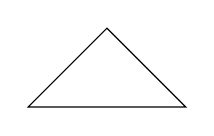
\begin{tikzpicture}
        \draw (0, 0) -- (1, 1) -- (2, 0) -- cycle;
    \end{tikzpicture}
\end{minted}

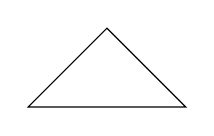
\begin{tikzpicture}
    \draw (0, 0) -- (1, 1) -- (2, 0) -- cycle;
\end{tikzpicture}
\newline

矩形、圆和椭圆:
\begin{minted}{LaTeX}
    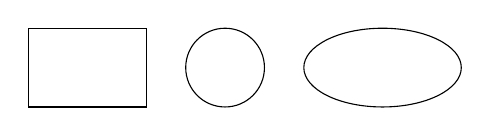
\begin{tikzpicture}
        \draw (0, 0) rectangle (1.5, 1);
        \draw (2.5, 0.5) circle[radius = 0.5];
        \draw (4.5, 0.5) ellipse[x radius = 1, y radius = 0.5];
    \end{tikzpicture}
\end{minted}

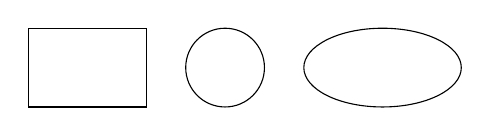
\begin{tikzpicture}
    \draw (0, 0) rectangle (1.5, 1);
    \draw (2.5, 0.5) circle[radius = 0.5];
    \draw (4.5, 0.5) ellipse[x radius = 1, y radius = 0.5];
\end{tikzpicture}
\newline

直角、圆弧、椭圆弧:
\begin{minted}{LaTeX}
    \begin{tikzpicture}
        \draw (0, 0) |- (1, 1);
        \draw (1, 0) -| (2, 1);
        \draw (4, 0) arc (0 : 135 : 1);
        \draw (6, 0) arc (0 : 135 : 1 and 0.5);
    \end{tikzpicture}
\end{minted}

\begin{tikzpicture}
    \draw (0, 0) |- (1, 1);
    \draw (1, 0) -| (2, 1);
    \draw (4, 0) arc (0 : 135 : 1);
    \draw (6, 0) arc (0 : 135 : 1 and 0.5);
\end{tikzpicture}
\newline

正弦、余弦曲线(四分之一个周期):
\begin{minted}{LaTeX}
    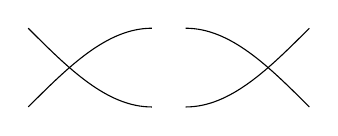
\begin{tikzpicture}
        \draw (0, 0) sin (1.57, 1);
        \draw (0, 1) sin (1.57, 0);
        \draw (2, 1) cos (3.57, 0);
        \draw (2, 0) cos (3.57, 1);
    \end{tikzpicture}
\end{minted}

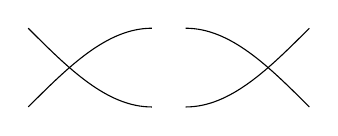
\begin{tikzpicture}
    \draw (0, 0) sin (1.57, 1);
    \draw (0, 1) sin (1.57, 0);
    \draw (2, 1) cos (3.57, 0);
    \draw (2, 0) cos (3.57, 1);
\end{tikzpicture}
\newline

抛物线(parabola),用 \texttt{bend} 控制顶点:
\begin{minted}{LaTeX}
    \begin{tikzpicture}
        \draw (0, 0) parabola (1, 2);
        \draw (2, 0) parabola bend (2.25, -0.25) (3, 2);
        \draw (4, 0) parabola bend (4.75, 2.25) (5, 2);
    \end{tikzpicture}
\end{minted}

\begin{tikzpicture}
    \draw (0, 0) parabola (1, 2);
    \draw (2, 0) parabola bend (2.25, -0.25) (3, 2);
    \draw (4, 0) parabola bend (4.75, 2.25) (5, 2);
\end{tikzpicture}
\newline

二次和三次贝塞尔曲线,分别使用一个和两个控制点:
\begin{minted}{LaTeX}
    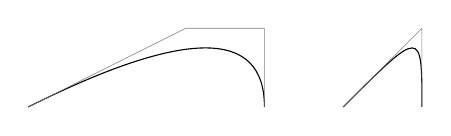
\begin{tikzpicture}
        \draw (0, 0) .. controls (2, 1) and (3, 1) .. (3, 0);
        \draw (4, 0) .. controls (5, 1) .. (5, 0);
        \draw[help lines] (0, 0) -- (2, 1) -- (3, 1) -- (3, 0)
            (4, 0) -- (5, 1) -- (5, 0);
    \end{tikzpicture}
\end{minted}

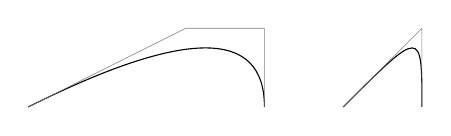
\begin{tikzpicture}
    \draw (0, 0) .. controls (2, 1) and (3, 1) .. (3, 0);
    \draw (4, 0) .. controls (5, 1) .. (5, 0);
    \draw[help lines] (0, 0) -- (2, 1) -- (3, 1) -- (3, 0)
        (4, 0) -- (5, 1) -- (5, 0);
\end{tikzpicture}
\newline

网格、函数图像,网格可用 \texttt{step} 参数控制网格大小,函数图像用 \texttt{domain} 参数控制定义域:
\begin{minted}{LaTeX}
    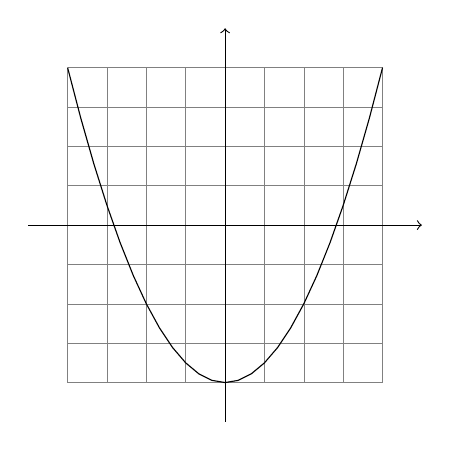
\begin{tikzpicture}
        \draw[help lines, step = 0.5] (-2, -2) grid (2, 2);
        \draw[->] (-2.5, 0) -- (2.5, 0);
        \draw[->] (0, -2.5) -- (0, 2.5);
        \draw[domain = -2 : 2] plot(\x, {\x * \x -2});
    \end{tikzpicture}
\end{minted}

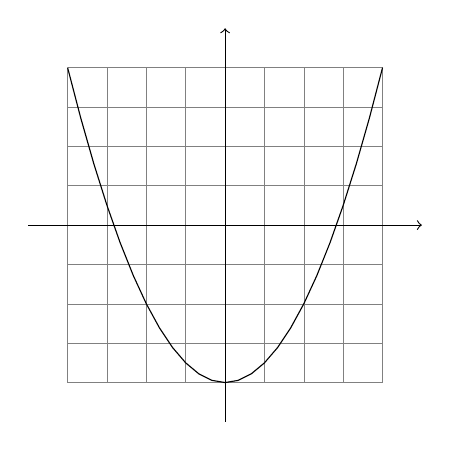
\begin{tikzpicture}
    \draw[help lines, step = 0.5] (-2, -2) grid (2, 2);
    \draw[->] (-2.5, 0) -- (2.5, 0);
    \draw[->] (0, -2.5) -- (0, 2.5);
    \draw[domain = -2 : 2] plot(\x, {\x * \x -2});
\end{tikzpicture}
\newline

\subsection{TikZ 绘图命令和参数}
除了 \mintinline{LaTeX}{\draw} 命令之外,TikZ 还提供了 \mintinline{LaTeX}{\fill} 命令来填充图形,
\mintinline{LaTeX}{\filldraw} 命令同时则同时填充和描边。除了矩形、圆等现成的闭合图形外,
\mintinline{LaTeX}{\fill} 和 \mintinline{LaTeX}{\filldraw} 命令也能够填充人为构造的闭合路径。

\begin{minted}{LaTeX}
    \draw[...] <path>;
    \fill[...] <path>;
    \filldraw[...] <path>;
\end{minted}

绘图参数可作为可选参数用在 \texttt{tikzpicture} 环境或 \mintinline{LaTeX}{\tikz} 命令时,参数会影响到所有具体
的绘图命令;用在单个绘图命令 \mintinline{LaTeX}{\draw}、\mintinline{LaTeX}{\filldraw} 等时,只对这个命令起效。

TikZ 还提供了 \texttt{scope} 环境,令一些绘图参数在局部起效:
\begin{minted}{LaTeX}
    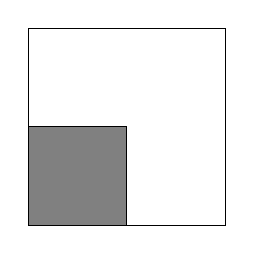
\begin{tikzpicture}
        \draw (0, 0) rectangle (2.5, 2.5);
        \begin{scope}[fill=gray, scale=0.5]
            \filldraw (0, 0) rectangle (2.5, 2.5);
        \end{scope}
    \end{tikzpicture}
\end{minted}

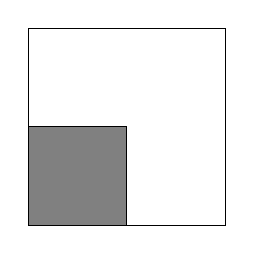
\begin{tikzpicture}
    \draw (0, 0) rectangle (2.5, 2.5);
    \begin{scope}[fill=gray, scale=0.5]
        \filldraw (0, 0) rectangle (2.5, 2.5);
    \end{scope}
\end{tikzpicture}

TikZ 有很多绘图参数,这些参数令 TikZ 能够绘制丰富多彩的图像,一些参数见表\ref{tab:tikz_draw_params}。

\begin{table}[H]
\caption{TikZ 常用的一些绘图参数}
\label{tab:tikz_draw_params}
\begin{center}
    \begin{itemize}
        \item \texttt{color=<color>} \\ 为线条(\mintinline{LaTeX}{\draw})或填充
        (\mintinline{LaTeX}{\fill})指定颜色,\emph{color} 使用颜色名或是 \texttt{xcolor} 的混合颜色语法。
        往往可以不写 \texttt{color=} 直接写颜色名称。
        \item \texttt{color=<color>} / \texttt{draw=<color>} \\ 分别给 \mintinline{LaTeX}{\filldraw}
        指定填充和描边的颜色。也可给 \mintinline{LaTeX}{\fill} 和 \mintinline{LaTeX}{\draw} 命令使用。不带
        参数直接使用 \texttt{fill} 和 \texttt{draw},相当于用默认颜色。
        \item \texttt{line width=<length>} \\ 指定线条粗细为 \emph{width}。默认普通线宽为 0.4pt。
        \item \texttt{thin / semithick / thick / ...} \\ 指定线条粗细为预定义的某个类型,默认为
        \texttt{thin}。总共有其中预定义的类型:\texttt{ultra thin}、\texttt{very thin}、\texttt{thin}、
        \texttt{thin}、\texttt{semithick}、\texttt{thick}、\texttt{very thick}、\texttt{ultra thick}。
        \item \texttt{help lines} \\ 指定线条为辅助线,相当于 \texttt{line width=0.2pt, gray}。
        \item \texttt{solid / dashed / dotted / dash dot / dash dot dot / ...} \\ 指定线条类型(实线、
        虚线等)。
        \item \texttt{rounded corners} \\ 将路径转向处绘制成圆角。可写成
        \texttt{rounded corners=<radius>} 使用给定的半径。
        \item \texttt{-> / -< / -to / -latex / -stealth / ...} \\ 指定路径终点的箭头种类。
        \item \texttt{<- / >- / to- / latex- / -stealth / ...} \\ 指定路径起点的箭头种类。起点和终点的箭头
        可以搭配,如 \texttt{<->} 或者 \texttt{latex-to} 等。
        \item \texttt{scale=<scale>} \\ 指定整个图像或某个路径的缩放比例。
        \item \texttt{xshift=<length> / yshift=<length>} \\ 指定整个图像或某个路径相对于原位置的水平/垂直
        位移。
        \item \texttt{rotate=<angle>} \\ 指定整个图像或某个路径旋转一定角度。
    \end{itemize}
\end{center}
\end{table}



\subsection{TikZ 文字结点}
TikZ 用 \mintinline{LaTeX}{\node} 命令绘制文字结点:
\begin{minted}{LaTeX}
    \node[options] (name) at (coordinate) {text};
\end{minted}

其中,\emph{name} 为结点命令,类似 \mintinline{LaTeX}{\coordinate};\texttt{at (coordinate)} 指定结点的位
置。这两者和前面的 \emph{options} 都可以省略,只有 \texttt{text} 是必填的。
\begin{minted}{LaTeX}
    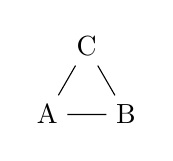
\begin{tikzpicture}
        \node (A) at (0, 0) {A};
        \node (B) at (1, 0) {B};
        \node (C) at (60 : 1) {C};
        \draw (A) -- (B) -- (C) -- (A);
    \end{tikzpicture}
\end{minted}

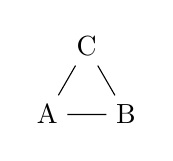
\begin{tikzpicture}
    \node (A) at (0, 0) {A};
    \node (B) at (1, 0) {B};
    \node (C) at (60 : 1) {C};
    \draw (A) -- (B) -- (C) -- (A);
\end{tikzpicture}

表~\ref{tab:tikz_draw_params} 中的参数可用于 \mintinline{LaTeX}{\node} 命令的配置。除此之外,
\mintinline{LaTeX}{\node} 还有一些特定的参数,见表~\ref{tab:tikz_node_params}。

\begin{table}[H]
\caption{TikZ 结点使用的一些绘图参数}
\label{tab:tikz_node_params}
\begin{center}
    \begin{itemize}
        \item \texttt{anchor=<position>} \\ 指定结点的某个角落 \emph{position} 位于给定的位置
        \emph{coordinate}。参数 \emph{position} 用 \texttt{center}、\texttt{north}、
        \texttt{north west} 等形式表示。
        \item \texttt{centered / above / below / left / right / above left / ...} \\ 指定结点相对于
        \emph{coordinate} 的位置,\texttt{anchor=<position>} 的等效写法。\texttt{above} 相当于
        \texttt{anchor=south},以此类推。带参数的形式 \texttt{above=<length>} 指定结点相对于
        \emph{coordinate} 的距离。
        \item \texttt{shape=<shape>} \\ 结点的形状,默认可用 \texttt{rectangle} 和 \texttt{circle},可省
        略 \texttt{shape=} 直接写。在环境前使用 \mintinline{LaTeX}|\usetikzlibrary{shapes.geometric}|
        命令可用更多的形状。
        \item \texttt{inner sep=<length> / outer sep=<length>} \\ 结点边界向外和向内的额外距离。
        \item \texttt{minimum size=<length> / minimum height=<length> / minimum width=<length>} \\
        结点的最小大小/高度/宽度。
        \item \texttt{text=<color>} \\ 结点文字的颜色。
        \item \texttt{node font=<font command>} \\ 结点文字的字体,形如 \mintinline{LaTeX}{\bfseries}
        或 \mintinline{LaTeX}{\itshape} 等。
    \end{itemize}
\end{center}
\end{table}

\mintinline{LaTeX}{\node} 命令不仅可以为文字结点的位置命名,在 \mintinline{LaTeX}{\draw} 等命令中还可以使用某
个结点的相对位置,以“东南西北”的方式命名:
\begin{minted}{LaTeX}
    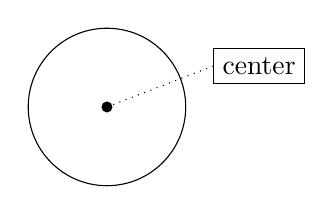
\begin{tikzpicture}
        \draw (0, 0) circle[radius=1];
        \fill (0, 0) circle[radius=2pt];
        \node[draw] (P) at (15 : 2) {center};
        \draw[dotted] (0, 0) -- (P.west);
    \end{tikzpicture}
\end{minted}

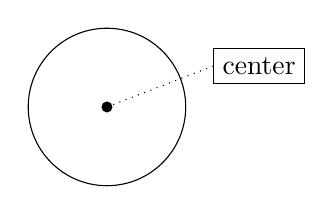
\begin{tikzpicture}
    \draw (0, 0) circle[radius=1];
    \fill (0, 0) circle[radius=2pt];
    \node[draw] (P) at (15 : 2) {center};
    \draw[dotted] (0, 0) -- (P.west);
\end{tikzpicture}
\newline

另一种用法是在 \mintinline{LaTeX}{\draw} 等命令的路径中使用 \texttt{node},不仅可以对某个位置标记结点,还能够对
线标记:
\begin{minted}{LaTeX}
    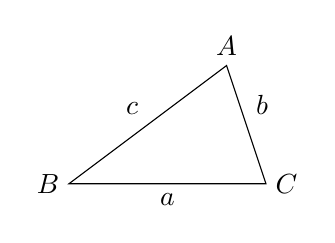
\begin{tikzpicture}
        \draw (2, 1.5) node[above] {$A$} -- node[above left] {$c$}
            (0, 0) node[left] {$B$} -- node[below] {$a$}
            (2.5, 0) node[right] {$C$} -- node[above right] {$b$} cycle; % cycle 令路径回到起点
    \end{tikzpicture}
\end{minted}

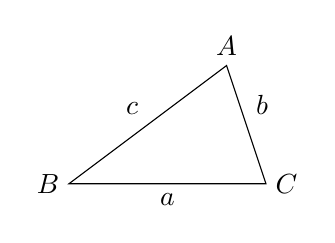
\begin{tikzpicture}
    \draw (2, 1.5) node[above] {$A$} -- node[above left] {$c$}
        (0, 0) node[left] {$B$} -- node[below] {$a$}
        (2.5, 0) node[right] {$C$} -- node[above right] {$b$} cycle; % cycle 令路径回到起点
\end{tikzpicture}
\newline

除了 \mintinline{LaTeX}{\node} 命令之外,\mintinline{LaTeX}{coordinate} 也可以通过参数为某个位置添加文
字(label)。下面是一个较为复杂的例子,综合前面的各种路径、形状、文字结点和参数设置:
\begin{minted}{LaTeX}
    \begin{tikzpicture}
        \draw[-stealth, line width=0.2pt] (-0.5, 0) -- (4.5, 0);
        \draw[-stealth, line width=0.2pt] (0, -0.5) -- (0, 2.5);
        \coordinate (a) at (0.5, 1.9);
        \coordinate (b) at (4, 1.2);
        \coordinate[label=below:$a$] (a0) at (a |- 0, 0);
        \coordiante[label=below:$b$] (b0) at (b |- 0, 0);
        \filldraw[fill=gray!20, draw, thick]
            (a0) -- (a) .. controls (1, 2.8) and (2.7, 0.4) .. (b) -- (b0) -- cycle;
        \node[above right, outer sep=0.2cm, rounded corners, fill=green!20, draw=gray,
            text=blue!60!black, scale=0.6]
            at (b) {$\displaystyle \int_a^b {f(x)\,\mathrm{d}x} = F(b) - F(a)$};
    \end{tikzpicture}
\end{minted}

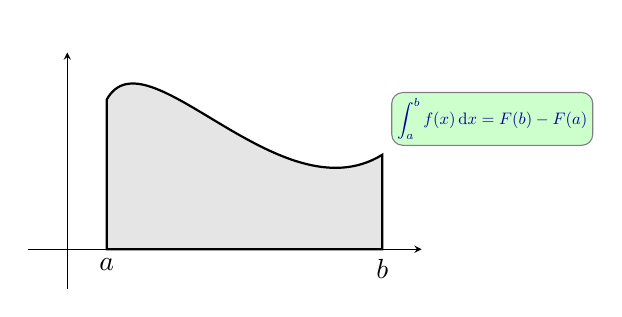
\begin{tikzpicture}
    \draw[-stealth, line width=0.2pt] (-0.5, 0) -- (4.5, 0);
    \draw[-stealth, line width=0.2pt] (0, -0.5) -- (0, 2.5);
    \coordinate (a) at (0.5, 1.9);
    \coordinate (b) at (4, 1.2);
    \coordinate[label=below:$a$] (a0) at (a |- 0, 0);
    \coordinate[label=below:$b$] (b0) at (b |- 0, 0);
    \filldraw[fill=gray!20, draw, thick]
        (a0) -- (a) .. controls (1, 2.8) and (2.7, 0.4) .. (b) -- (b0) -- cycle;
    \node[above right, outer sep=0.2cm, rounded corners, fill=green!20, draw=gray,
        text=blue!60!black, scale=0.6]
        at (b) {$\displaystyle \int_a^b {f(x)\,\mathrm{d}x} = F(b) - F(a)$};
\end{tikzpicture}

\subsection{TikZ 其他的一些示例}
弧和扇形:
\begin{minted}{LaTeX}
    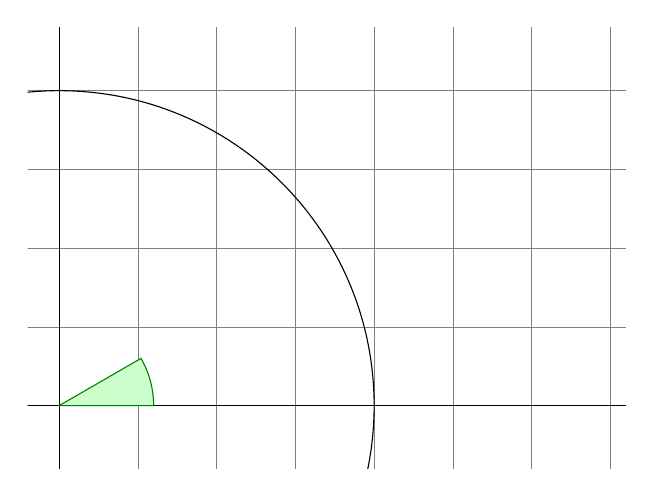
\begin{tikzpicture}
        \clip (-0.4, -0.8) rectangle (7.2, 4.8);
        \draw[step=1cm, gray, very thin] (-5.6, -5.6) grid (13.6, 13.6);
        \draw (-6.0, 0) -- (10.0, 0);
        \draw (0, -6.0) -- (0, 6.0);
        \draw (0, 0) circle (4cm);
        \filldraw[fill=green!20!white, draw=green!50!black]
            (0, 0) -- (12mm, 0mm) arc (0 : 30 : 12mm) -- cycle;
    \end{tikzpicture}
\end{minted}

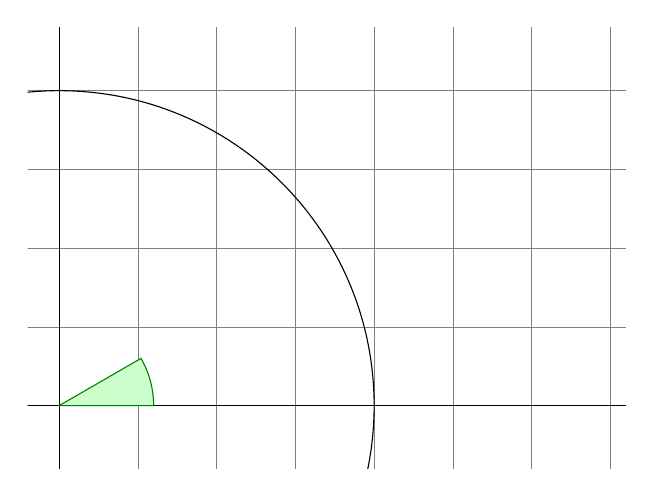
\begin{tikzpicture}
    \clip (-0.4, -0.8) rectangle (7.2, 4.8);
    \draw[step=1cm, gray, very thin] (-5.6, -5.6) grid (13.6, 13.6);
    \draw (-6.0, 0) -- (10.0, 0);
    \draw (0, -6.0) -- (0, 6.0);
    \draw (0, 0) circle (4cm);
    \filldraw[fill=green!20!white, draw=green!50!black]
        (0, 0) -- (12mm, 0mm) arc (0 : 30 : 12mm) -- cycle;
\end{tikzpicture}
\newline

简单的维恩图(Venn diagram):
\begin{minted}{LaTeX}
    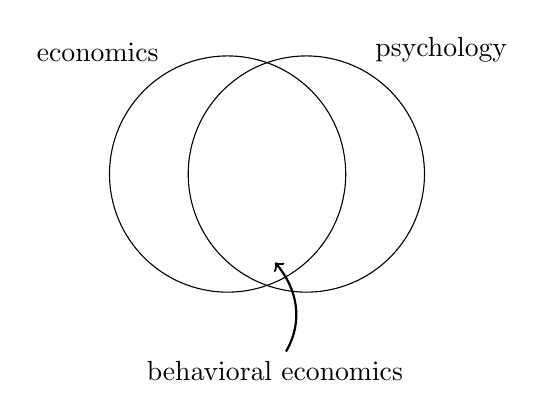
\begin{tikzpicture}
        \node[circle, draw, minimum size=3cm, label=120:{economics}]
            at (0, 0) {};
        \node[circle, draw, minimum size=3cm, label=60:{psychology}]
            at (1, 0) {};
        \node (i) at (0.5, -1) {};
        \node at (0.6, -2.5) {behavioral economics}
            edge[->, thick, out=60, in=-50] (i);
    \end{tikzpicture}
\end{minted}

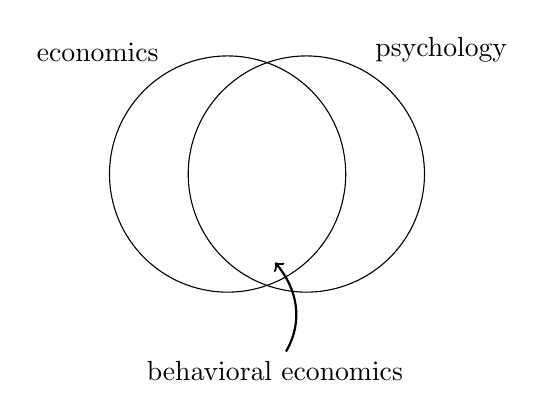
\begin{tikzpicture}
    \node[circle, draw, minimum size=3cm, label=120:{economics}]
        at (0, 0) {};
    \node[circle, draw, minimum size=3cm, label=60:{psychology}]
        at (1, 0) {};
    \node (i) at (0.5, -1) {};
    \node at (0.6, -2.5) {behavioral economics}
        edge[->, thick, out=60, in=-50] (i);
\end{tikzpicture}
\newline

\texttt{foreach} 循环:
\begin{minted}{LaTeX}
    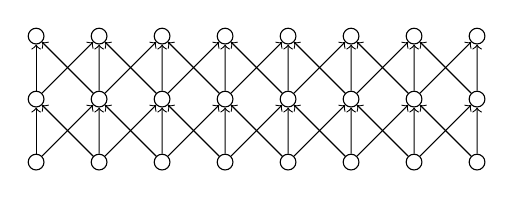
\begin{tikzpicture}[scale=0.8]
        \tikzstyle{v}=[circle, minimum size=2mm, inner sep=0pt, draw]
        \foreach \i in {1, ..., 8}
            \foreach \j in {1, ..., 3}
                \node[v] (G-\i-\j) at (\i, \j) {};
        \foreach \i in {1, ..., 8}
            \foreach \j/\o in {1/2, 2/3}
                \draw[->] (G-\i-\j) -- (G-\i-\o);
        \foreach \i/\n in {1/2, 2/3, 3/4, 4/5, 5/6, 6/7, 7/8}
            \foreach \j/\o in {1/2, 2/3} {
                \draw[->] (G-\i-\j) -- (G-\n-\o);
                \draw[->] (G-\n-\j) -- (G-\i-\o);
            }
    \end{tikzpicture}
\end{minted}

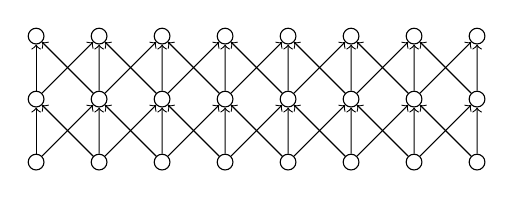
\begin{tikzpicture}[scale=0.8]
    \tikzstyle{v}=[circle, minimum size=2mm, inner sep=0pt, draw]
    \foreach \i in {1, ..., 8}
        \foreach \j in {1, ..., 3}
            \node[v] (G-\i-\j) at (\i, \j) {};
    \foreach \i in {1, ..., 8}
        \foreach \j/\o in {1/2, 2/3}
            \draw[->] (G-\i-\j) -- (G-\i-\o);
    \foreach \i/\n in {1/2, 2/3, 3/4, 4/5, 5/6, 6/7, 7/8}
        \foreach \j/\o in {1/2, 2/3} {
            \draw[->] (G-\i-\j) -- (G-\n-\o);
            \draw[->] (G-\n-\j) -- (G-\i-\o);
        }
\end{tikzpicture}
\newline

如果在 \texttt{tikzpicture} 环境前使用 \mintinline{LaTeX}{\usetikzlibrary} 命令,name 就可以启用更多的附加功能,可以画出更特殊的形
状,就像下面的有些弯曲的盒子:
\begin{minted}{LaTeX}
    \usetikzlibrary{decorations.pathmorphing}
    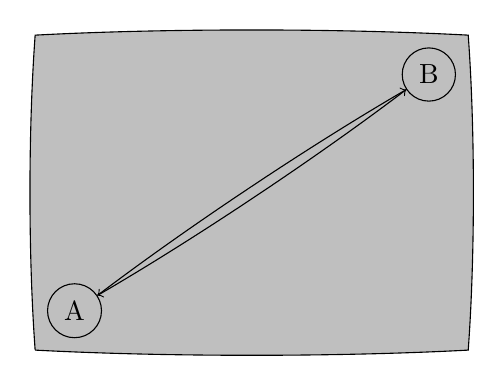
\begin{tikzpicture}[decoration={bent, aspect=.3}]
        \draw[decorate, fill=lightgray] (0, 0) rectangle (5.5, 4);
        \node[circle, draw] (A) at (.5, .5) {A};
        \node[circle, draw] (B) at (5, 3.5) {B};
        \draw[->, decorate] (A) -- (B);
        \draw[->, decorate] (B) -- (A);
    \end{tikzpicture}
\end{minted}

\usetikzlibrary{decorations.pathmorphing}
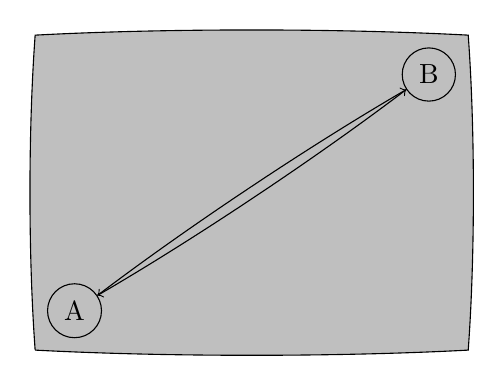
\begin{tikzpicture}[decoration={bent, aspect=.3}]
    \draw[decorate, fill=lightgray] (0, 0) rectangle (5.5, 4);
    \node[circle, draw] (A) at (.5, .5) {A};
    \node[circle, draw] (B) at (5, 3.5) {B};
    \draw[->, decorate] (A) -- (B);
    \draw[->, decorate] (B) -- (A);
\end{tikzpicture}
\newline

带圈的文字结点图:
\begin{minted}{LaTeX}
    \usetikzlibrary{positioning}
    \begin{tikzpicture}[xscale=6, yscale=8, >=stealth]
        \tikzstyle{v}=[circle, minimum size=1mm, draw, thick]
        \node[v] (a) {$1$};
        \node[v] (b) [right=of a] {$2$};
        \node[v] (c) [below=of a] {$2$};
        \node[v] (d) [below=of b] {$1$};
        \draw[thick, ->] (a) to node {} (c);
        \draw[thick, ->] (a) to node {} (d);
        \draw[thick, ->] (b) to node {} (d);
    \end{tikzpicture}
\end{minted}

\usetikzlibrary{positioning}
\begin{tikzpicture}[xscale=6, yscale=8, >=stealth]
    \tikzstyle{v}=[circle, minimum size=1mm, draw, thick]
    \node[v] (a) {$1$};
    \node[v] (b) [right=of a] {$2$};
    \node[v] (c) [below=of a] {$2$};
    \node[v] (d) [below=of b] {$1$};
    \draw[thick, ->] (a) to node {} (c);
    \draw[thick, ->] (a) to node {} (d);
    \draw[thick, ->] (b) to node {} (d);
\end{tikzpicture}
\newline

甚至可以用 TikZ 来画一些语法图,就好像是排版书籍时用 Pascal 语言编写输出的一样。但是代码比上面的例子要复杂很多,
\texttt{pgf} 宏包的文档里有一些介绍。

如果必须要画一些数值数据或者数学方程的图像,可以用 \texttt{pgfplot} 宏包,它提供了你所有在画图时需要的东西,甚至可以
调用 \texttt{gnuplot} 命令验证它画出的函数图像都没问题。

此外,在 \TeX ample.net 上有一些关于 TikZ/PGF 的工具,所以不需要把所有的代码都敲一遍。


\end{document}
